\section{System Architecture and Methods}
\label{sec:System Architecture and Methods}
This triple-heterogeneous software stack follows a high performance middleware design pattern,
focusing its structure on the orchestration of distributed classical resources alongside remote, cloud based quantum backends. The stack 
addresses the preestablished CPU-QPU bottleneck \parencite{cruise2020practicalquantumcomputingvalue} through the development of an asynchronous and 
parallelized pipeline, designed to be resuable middleware running unchanged across CPU, GPU, QPU backends 
instead of as a single purpose research script. Validation is conducted by executing the 
hybrid quantum-classical VQE software to find the ground state energies of the HWE ansatz VQE benchmark molecules from the previous work of 
\textcite{kandala2017hardware}'s: $H_2, LiH, BeH_{2}$, extended to $H_{2}O$, $NH_{3}$, and $N_{2}$, providing a    
measurable speedup when compared to the serial, nondistributed Qiskit baseline while remaining competivie against distributed statevector 
baselines without requiring users to abandon their existing simulator stacks. 

\subsection{Distributed System Architecture}
This stack follows a modular architecture, designed to decouple the classical, high performance subroutines of SPSA optimization, Pauli term evaluation, local statevector
construction, and the distributed MPI coordination from the quantum circuit execution and measurement of expectation values, allowing for the asynchronous execution of each. 
Three distinct layers are defined within the architecture: the Orchestration layer, the Acceleration layer, and the Quantum interface layer. 
This decomposition is needed due to each component operating across five orders of magnitude of timescales:
GPU accelerated classical math (microseconds), MPI internode communication (milliseconds), and the cloud based 
QPU Round-Trip Time (RTT)(seconds). Without decoupling, we would face the slowerest layer (QPU RTT) serializing and stalling the 
classical computation, rather than allowing it to overlap. Compared to full HPC integrated hybrid workflow platforms such as JHPC-Quantum \parencite{shehata2026openqse},
which instead supports distributed execution while requiring per-target manual configuration (as opposed to this stacks offered automatic 
hardware detection and single run CPU+GPU+QPU integration). 

\begin{figure*}[htbp]
    \centering
    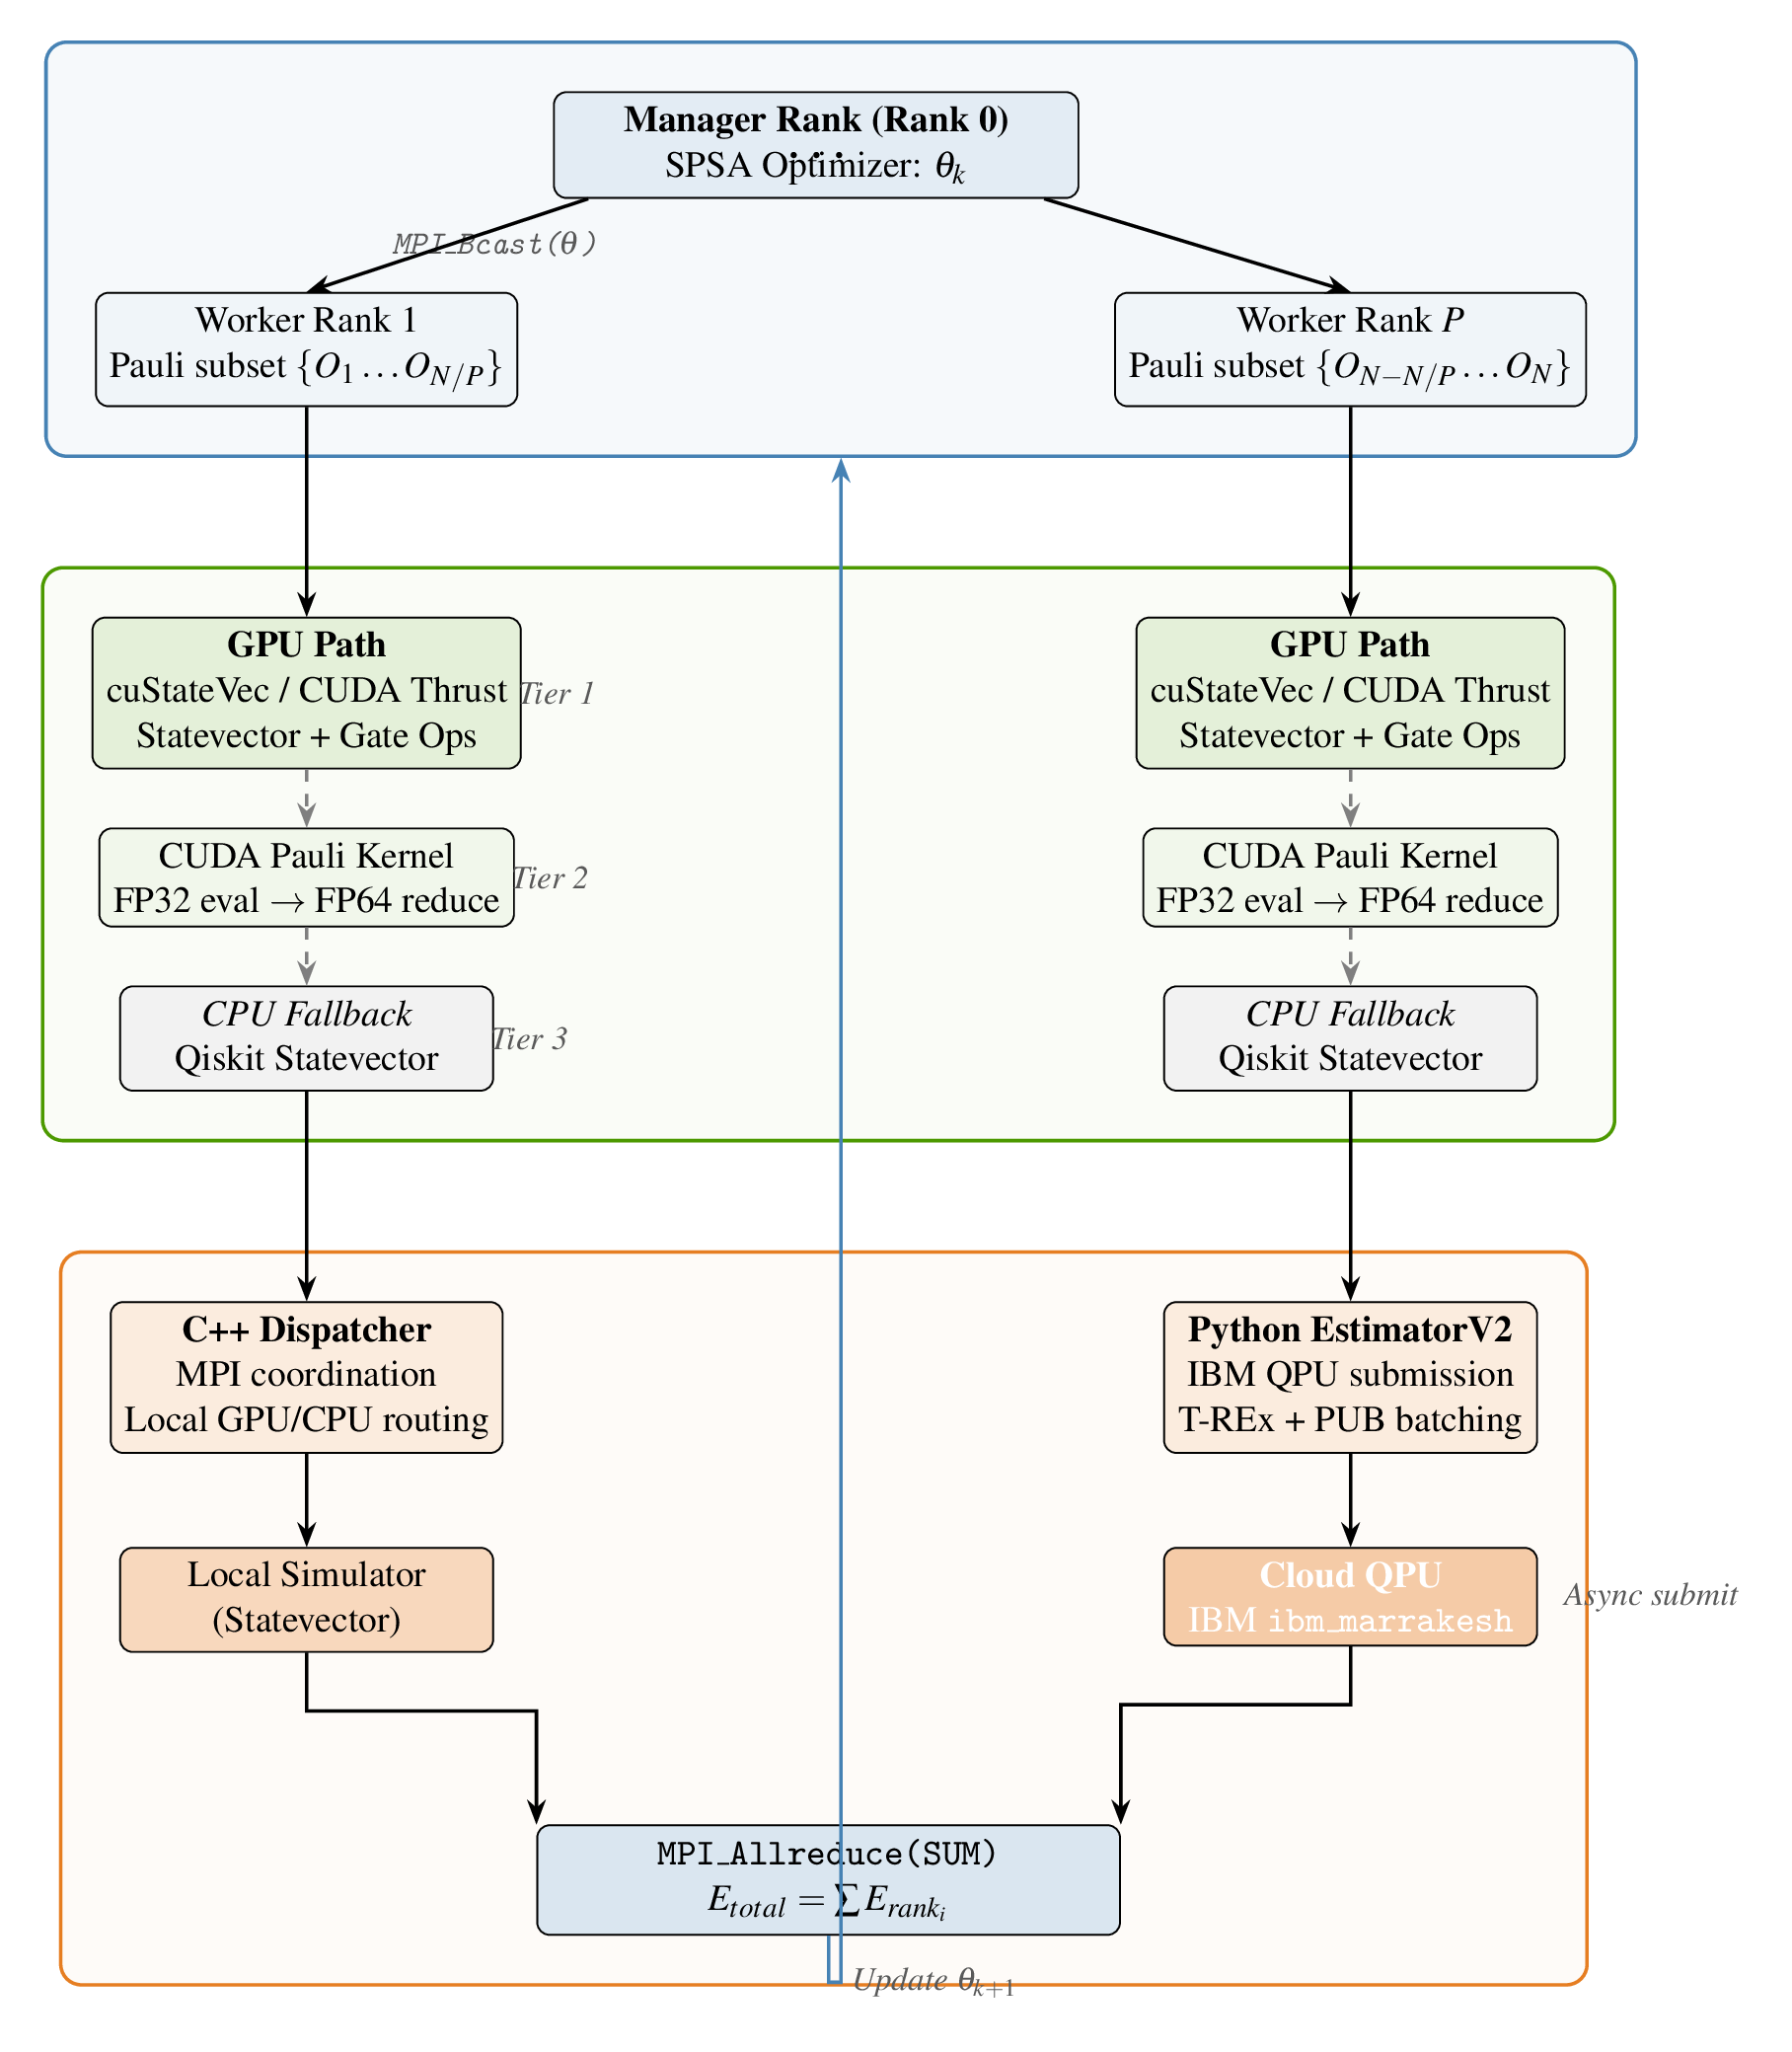
\includegraphics[width=0.65\textwidth]{graphics/system_arch_diagram.png}
    \caption{Triple Heterogeneous System Architecture.}
    \label{fig:system_architecture}
\end{figure*}

\subsubsection{Orchestration Layer: Distributed Memory and MPI Manager-Worker Topology}
This top-level layer implements a manager-worker topology that utilizes Message Passing Interface (MPI)
to manage MPI ranks (workers). The manager rank (rank 0) holds the global 
state of the classical optimizer SPSA, the current $\theta$ variational parameter vector, determining the pertubed values of $\theta^+$ and $\theta^-$, and then distributing the 
$\theta$ sets across the ranks of available classical workers to enable concurrent gradient 
estimation. SPSA is a derivative-free optimizer, found well suited to handle the quantum measurement noise on 
physical qubits (unlike the gradient based methods of Adam or SGD) \parencite{pellow2021classicoptimizers}, which 
makes SPSA the optimal choice on NISQ hardware to manage the physical, noisy objective functions. 
    
By utilizing \texttt{MPI\_Ibcast} in the C++ dispatcher and \texttt{comm.Bcast} and \texttt{comm.Allreduce} in the Python path for the same role, the stack enables communication between the 
classical-quantum components. Within the Python path, the overlp between QPU wait times and classical compuation is achieved, not through non-blocking MPI primitives but instead by code restructuring: 
QPU jobs are submitted and its result deferred while ranks proceed with the local statevector work, with the only blocking
occurs on \texttt{job.result()} once local work is completed. Once worker ranks receive the expectation values, they 
execute a \texttt{MPI\_allreduce} aggregation for each rank's partial energy to then update the global objective function. 

\begin{figure*}[htbp]
    \centering
    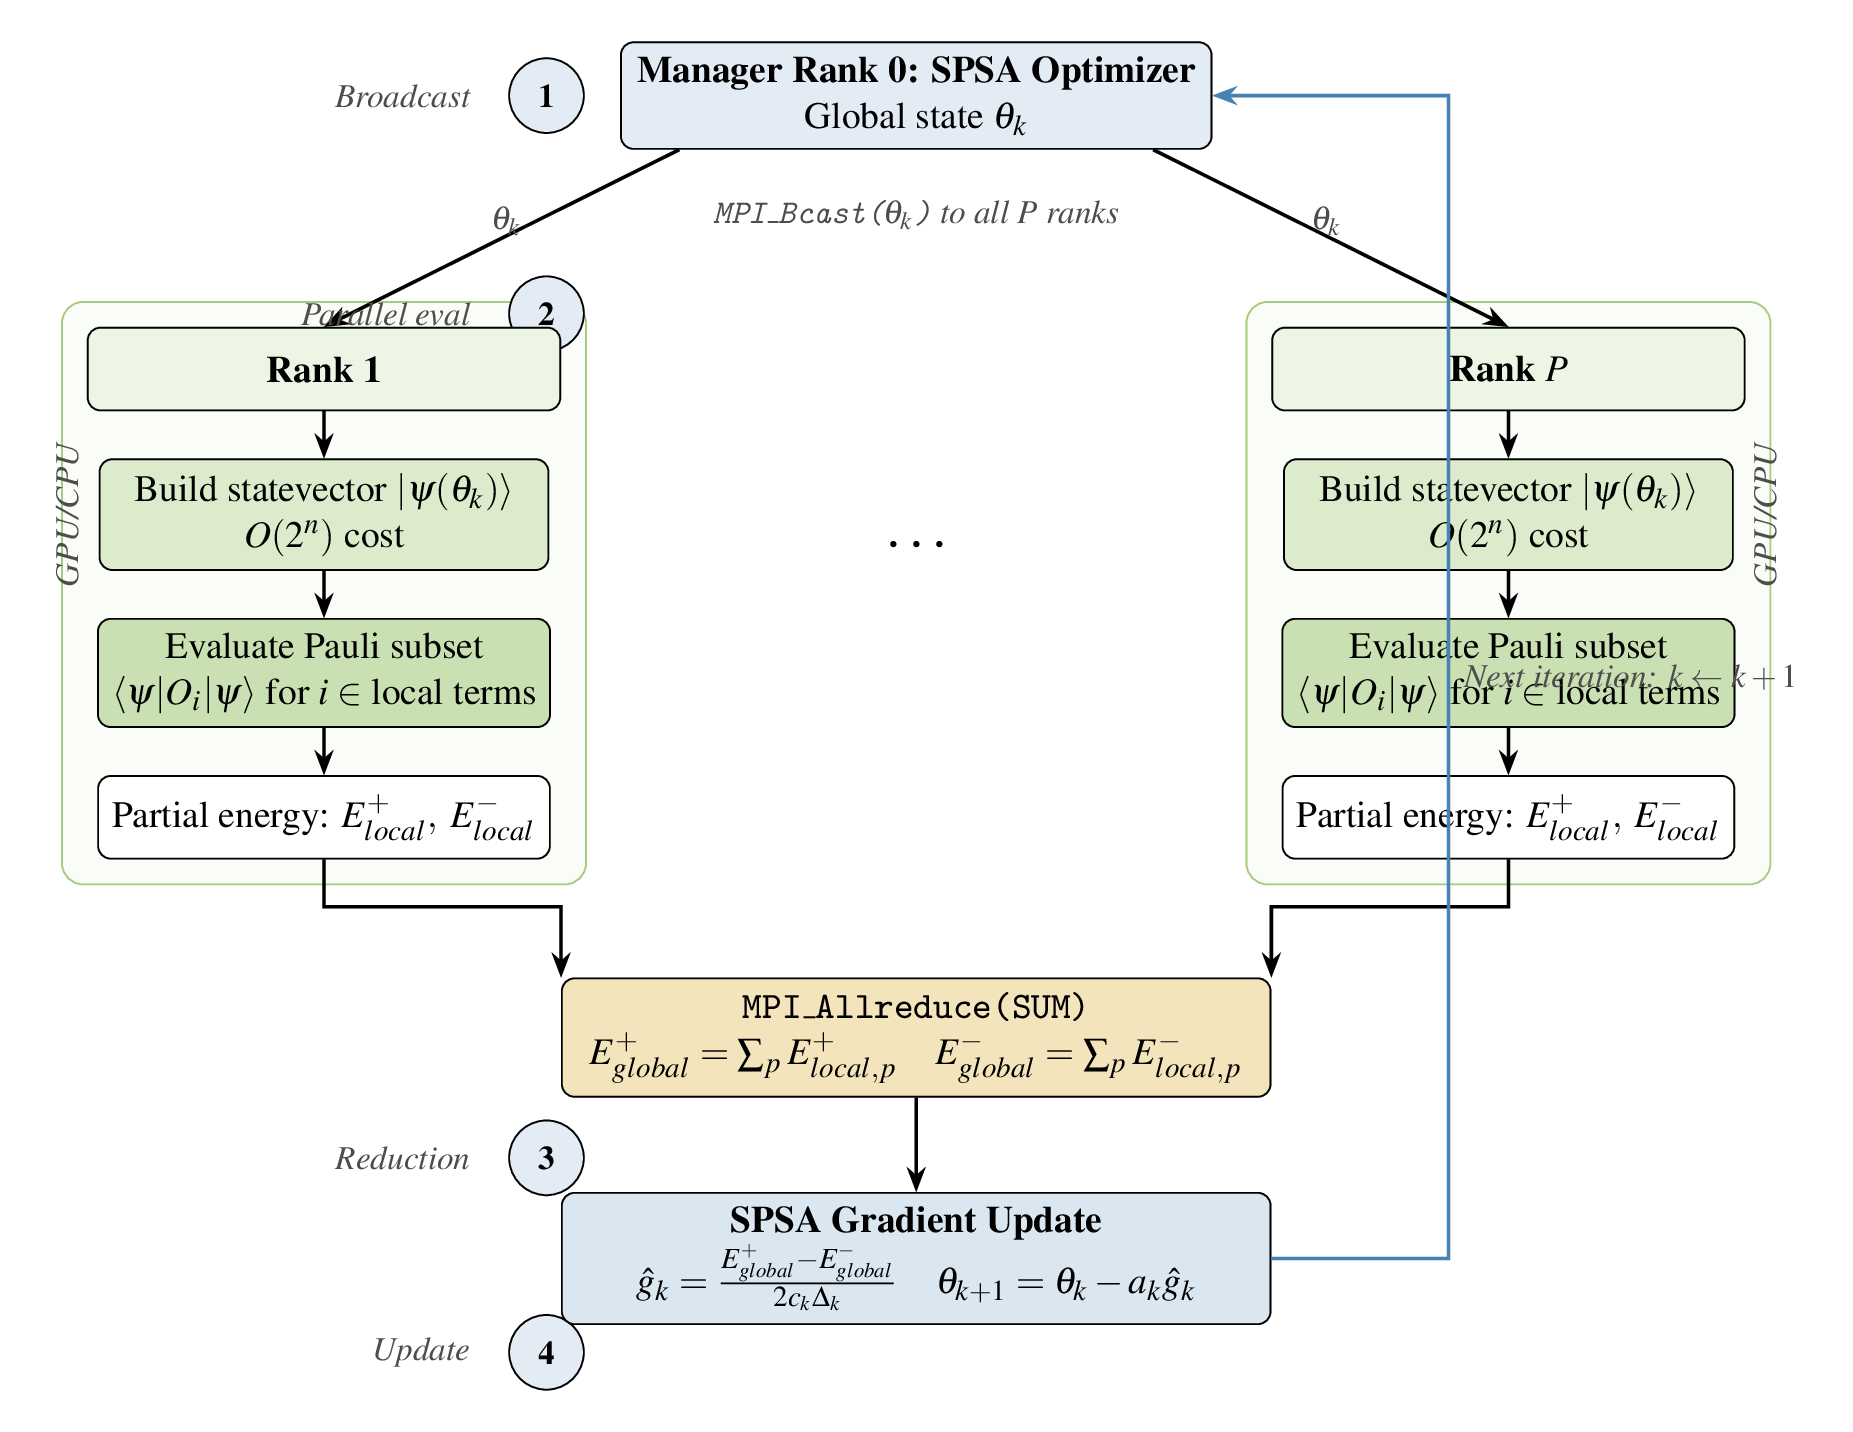
\includegraphics[width=0.65\textwidth]{graphics/spsa_topology.png}
    \caption{Distributed SPSA Topology}
    \label{fig:spsa_topology}
\end{figure*}

\subsubsection{Acceleration Layer: Intra-Process CUDA-Kernel Execution}
This layer follows the findings of \textcite{bayraktar2023cuquantum}, with the design
offloading the computationally heavy $2^n$ state-vector math to each MPI rank's NVIDIA GPU. The stack selects between
two accelerated processing options, autodectected at runtime: 
\begin{enumerate}
    \item \textbf{GPU statevector (cuStateVec)}: Best option, used when an NVIDIA GPU is detected. The stack switches to Qiskit Aer's GPU-accelerated statevector simulator backed by NVIDIA's cuStateVec library from the cuQuantum SDK. This accelerates the $O(2^n)$ local statevector construction, which dominates per-iteration cost \parencite{bayraktar2023cuquantum}, along with all gate operations (CNOT, rotations) being executed as GPU matrix multiplications.
    \item \textbf{CPU fallback}: When no GPU is available, the stack falls back to Qiskit's CPU-based Python/C++ \texttt{Statevector} class for exact (noiseless) state-vector simulation. 
\end{enumerate}

With the GPU path, the stack applies an automatic mixed-precision strategy using FP32/FP64 to balance the stack's need 
for high computational throughput with the need for numerical accuracy. When solving problems under 20 qubits, both consumer and workstation-grade GPUs 
use FP32 (Single Precision) statevector representation, exploiting the relatively low FP64:FP32 throughput ratio of these cards to gain a 
substantial free throughput speedup. Datacenter class GPUs (A100s, H100s) and any problems >= 20 qubits use FP64 (Double Precision), where the throughput 
asymmetry across the precisions is smaller and preciseness is preferred. This choice is resolved once per problem by \texttt{HardwareProfile.recommend_precision()} but can
be overriden explicitly by the user (\texttt{VQE_PRECISION=fp32\textbar fp64}). Within this paper, every result reporterd was produced
through one of these acceleration paths. A third, experimental path exists within the codebase, containing a custom CUDA kernel for Pauli-term expectation value with an 
independent FP32/FP64 mixed precision split, described futher in \S[Future Work], but is not wihtin the autoselection and does not contribute to any published results.  

% precise, used to handle the trigonometric computations of \texttt{cosf} and \texttt{sinf} within each Pauli term evaluation (only needing 7 decimal digits of precision), which provides up to 2x faster throughput 
% on the GPU cores. FP64 (Double Precision), the slower but exact option, is used in the tree reduction and global accumulation phases in 
% order to prevent precision loss (rounding errors) that can occur during the MPI \texttt{Allreduce} 
% aggregation. This combination is to maintain chemical accuracy while reducing the memory bandwidth bottleneck recognized by
% \textcite{bayraktar2023cuquantum} within state vector simulation due to reading/writing the statevectors from GPU memory instead of the floating point computation.

\subsubsection{Quantum Interface Layer - Asynchronous Dispatcher}
This layer is the bottom of the stack, handling the abstraction of how quantum hardware-specific drivers 
(or simulators) perform computations while allowing the previous layers to function regardless if they 
are using a local simulator (CPU), local GPU, or a cloud GPU. This setup extends the core ideas of XACC's accelerator model \parencite{mccaskey2018xacc}.   
Two dispatch paths occur:
\begin{enumerate}
    \item \textbf{C++ dispatcher} (\texttt{dispatcher.cpp}): Manages the MPI synchronization with rank 0 using \texttt{MPI\_Ibcast} for $\theta$  parameter distribution and \texttt{MPI\_Allreduce} for partial energy aggregation from all ranks (later to be broadcasted). Local routes computation (to either CUDA Pauli kernel or to CPU mean-field fallback path) is the same diagnostic-only path previously mentioned in \S Acceleration Layer and does not contribute to the results of this paper. In the seperate, complete cloud IBM QPU path, \texttt{std::async} is used for nonblocking job submission via a launched REST client on a background thread, ensuring main thread does not block, while (\texttt{qpu\_client.cpp}) handles IBM Quantum's IAM authentication, JSON payload construction, and polling with exponential backoff (starting at 2s, doubling until 30s). While this path is fully implemented, it was not used within reported experiments either, in favor of the Python EstimatorV2 path, remaining instead as a candidate route for future, low-level QPU integration work. 
    \item \textbf{Python EstimatorV2 path} (\texttt{interface.py}): For IBM Quantum experiments, the stack uses Qiskit's EstimatorV2 primitive, providing the stack with built-in transpilation, observable layout mapping, and with T-REx measurement error mitigation for NISQ hardware \parencite{cai2023quantumerrormitigation}. As SPSA requires both $E(\theta^+)$ and $E(\theta^-)$ gradient estimations per iteration \parencite{pellow2021classicoptimizers}, these get bundled into a single job as two Primitive Unified Blocs (PUBs), therefore halving the number of QPU round-trips. During the QPU wait time, all MPI ranks independently compute exact statevector expectation values, providing both noise-free reference estimate and useful classical work that contributes to the masking metric $M$.
\end{enumerate}

Every reported result within this paper utilzies the Python EstimatorV2 path for QPU access and the GPU statevector/CPU fallback paths
(as described within \S Acceleration Layer for local computation). The C++ dispatcher path remainds as a documented, implemented alternative, 
with its QPU submission path production-ready and only left unused by choice, while the local compute routing would require the physics fix described 
in \S Future work before being trusted for published results. 

% SMART TO KEEP MENTIONING THIS ROUTE NOT WORKING? SHOULD I LIMIT IT TO FUTURE WORK INSTEAD, AS I FEEL IT DISCREDITS THE FUNCTIONALITY OF MY STACK TOO EARLY ON? 




\subsection{Algorithmic Workflow: Parallelized VQE}
The VQE algorithm is reformulated in this stack from \textcite{peruzzo2014variational}'s single host VQE, in order to exploit its distributed nature, 
following an iterative cycle of: 
    \begin{enumerate}
        \item \textbf{Global Parameter Broadcast}: The optimizer rank broadcasts a vector of parameters ($\theta$) to $P$ parallel ranks.
        \item \textbf{Parallel Expectation Value Estimation}: Each rank ($p \in P$) computes its assigned subset of the Pauli string expectation values: $$\langle\psi(\theta)|\hat{O}_i|\psi(\theta)\rangle$$, with $O_i$ terms partitioned across the MPI ranks. This is the stack's primary point of task parallelization, with the distribution of independent Pauli-term evaluations instead of relying on a single global reduction \parencite{bayraktar2023cuquantum}.
        \item \textbf{Asynchronous Handshake}: When using the cloud QPU backend, circuits queue on the remote processor while the classical MPI ranks will independently compute the exact statevector expectation values locally. This overlap provides both noise-free reference estimate and classical work that masks the QPU round-trip latencies.
        \item \textbf{Reduction and Updating}: Partial expectation values from all ranks get aggregated using \texttt{MPI\_Allreduce} into a single energy sum, which the classical gradient-free optimizer SPSA \parencite{pellow2021classicoptimizers} uses (alongside the perturbed $E(\theta^+)$ and $E(\theta^-)$) to compute the next $\theta$ for the following iteration.
    \end{enumerate}


\subsection{Performance Evaluation and Experimental Design}
This section describes the full evaluation of this middleware stack validated through a Strong Scaling analysis, where the
total problem size is kept fixed at LiH (12 qubits) while the number of cores increases, in order to determine points of speedup \parencite{cuboulderScaling}. This method of
analysis is crucial to determing how to exploit the full potential of parallelizing the workload and at what point additional processors are no longer beneficial.
This measurement is governed by Amdahl's Law \parencite{amdahl1967validity},
to calculate the maximum (theoretical) speedup of a parallel system, establishing the threshold where adding processors will yield diminishing returns.
A Weak Scaling analysis was also implemented, with the molecular complexity grows proportionally with the number of ranks from $H_2$ at $P{=}1$ to $H_{2}O$ at $P{=}8$ (aiming for roughly constant Pauli term counts per rank), testing if the per-iteration wall-clock time
remains stable while the workload scales, as established in the work of \textcite{gustafson1988reevaluating}.
Both analyses were conducted to test the ability of the stack's GPU-accelerated path to scale both in 
its parallelization efficiency and its ability in handling increasingly larger, more complex molecular workloads. 


\subsubsection{Experimental Configuration}  
All simulator experiments of this stack were conducted inside a Docker container (CUDA toolkit 12.6.3, Qiskit $\geq$2.5.2, qiskit-ibm-runtime $\geq$0.49.0, Python 3.11, PySCF $\geq$2.14.0, OpenMPI from Ubuntu 22.04 system package) on a NVIDIA A100-SXM4-40GB (Lamdba Cloud), the primary validated hardware target of the stack.
% on a single host machine (a standard laptop setup, reflecting modern day hybrid quantum communication) Intel Core i7-1065G7 (Ice Lake, with 4 physical cores, 8 logical threads) clocked at 1.30 GHz base, 3.90 GHz turbo with 32 GB RAM,running on a Linux Mint OS. 
This configuration is set to ensure reproducibility across computing devices, demonstrating its portability and capacity to scale from commodity hardware up to datacenter-class GPUs. The same containerzied
Docker environment is reproducible on any host, regardless of the GPU utilzied. Wall-clock times are aggregated across $n=5$ independent random SPSA seeds ($n=10$ for LiH due to its bimodal convergence behavior),
reported as the median of the seeds with [min, max] range, using \texttt{benchmarks/aggregate_seeds.py} .

This middleware utilizes the VQE algorithm configured with tiered system that selects an ansatz based on a correlation score metric, computed
from each introduced molecules Pauli-term structure. All 6 benchmark molecules ($H_{2}O$, $LiH$, $BeH_{2}$, $H_{2}O$, $NH_{3}$, $N_{2}$) all fall within the \texttt{hwe_adaptive}
tier as the correlation scores fall between 0.34-0.50, where notably, none reach the 0.55 threshold that would then trigger the particle conserving UCCSD tier (despite the six-fold range within the set in qubit 
counts and Pauli-term complexity). The Shallow, HWE (hardware-efficient) ansatz ensures rapid computations on shallow circuits along with the classical optimizer SPSA, 
effective for navigating quantum noise found on NISQ devices, following \textcite{kandala2017hardware}'s setup with an expansion to dispatching to a GPU accelerated dispatch for an enhanced computational speedup.  
SPSA has a set fixed perturbation size $c = 0.1$ that can appropriately handle variational 
angles within $[0,2\pi]$ with a step size of $a=0.628 / \sqrt{p/8}$, which scales inversely with the square root of the 
number of variational parameters. The stability constant, $A = 0.1 \times \text{max\_iterations}$ delays any aggressively early 
updates while the decay exponents of $\alpha= 0.602$ and $\gamma = 0.101$ follow the standard schedule of SPSA. The per-iteration update rule is:
\begin{equation}
    a_k = \frac{a}{(k + A)^\alpha}, \quad c_k = \frac{c}{k^\gamma}
\end{equation}
Convergence is determined by a sliding window of 10 iterations and the SPSA optimizer terminates when $\max(E)-\min(E) < \tau$ occurs 
within that window (as $\tau = 1.6$ mHa, the chemical accuracy threshold defined in this stack). An enforced minimum iteration count of $\max(10, \min(2p, 50))$ 
is applied to prevent false convergences from occurring on the small, early steps. A maximum iteration count scales alongside 
the number of parameters with $\max(200, 8p)$. For reproducibility, all experiments use a fixed random seed of 42. 

All quantum backend experiments utilize IBM Quantum’s open access plan, which provides free access to the 156 qubit \texttt{ibm\_marrakesh} production-scale processor without a financial barrier for research. IBM Quantum was selected as this stack's cloud QPU provider due 
to their Qiskit library providing the means for effective hybrid middleware integration, offering the EstimatorV2 primitive with built-in source code language conversion and error mitigation \parencite{rallis2025interfacingquantumcomputingsystems}.  
In this stack, the Qiskit IBM Runtime EstimatorV2 primitive is configured with 4096 shots per circuit and with a resilience level 1 (T-REx measurement error mitigation) in order to balance the precision $1/\sqrt{4096} \approx 0.016\;E_h$ per expectation value while 
operating within the time limits of the IBM open access plan. 
The GPU-accelerated experiments are conducted on an NVIDIA A100-SXM4-40GB (Lambda Cloud),
using both the Qiskit Aer CUDA thrust backend and the NVIDIA cuStateVec backend to accelerate the construction of the state vector and the local GPU gate operations. This datacenter-grade GPU provides high memory bandwidth (1,555 GB/s) as the primary driver to the measured strong-scaling results
(\S[Results]) as the statevector simulation is memory bandwidth bound \parencite{bayraktar2023cuquantum}. The auto-detecion layer (\texttt{HardwareProfile}) allows for the same codebase to run unchanged on lower tier consumer 
and workstation GPUs, with an automatic adjustment of the precision policy (\S[Acceleration Layer]). While A100s are the sole GPU class reported within this paper, this 
portability was validated across the hardware ladder during the stack development. 


\subsubsection{Application Scenarios}
To demonstrate the effectiveness of this middleware when tasked a scientifically meaningful workload, this paper focuses on testing 
quantum chemistry, specifically the computation of the molecular electronic ground-state energies of six increasingly complex molecules over the iterations of the VQE. Chemistry was selected to be the  
application for this middleware due to three main reasons: 
    \begin{enumerate}
        \item Molecular Hamiltonians (mathematical description of electron interactions) map naturally to a qubit operator ($X$,$Y$,$Z$,$I$) through the Jordan-Wigner transformation \parencite{peruzzo2014variational}, which produces a clearly defined set of Pauli terms (ranging from 15 for $H_2$ to 3057 for $NH_{3}$) to then be batched and distributed across MPI ranks (while still not exceeding the coherency limitations of modern day QPUs). If this stack extended to operate beyond chemistry into fields such as finance or logistics, the decomposition into distributed subsets is not as straightforward. 
        \item Problem size scales predictably with the number of electrons and basis functions to allow for controlled experiments (ranging from 4-20 qubits as the benchmark scales from $H_2 - N_2$). This allows testing the stack with Strong/Weak scaling analyses.  
        \item Preexisting Full Configuration Interaction (FCI) energies provides a comparison to a verified, exact ground-truth references for each molecule's $E_0$ \parencite{szabo1996modernquantumchemistry}, in order to evaluate the stack's ability to maintain an approximate chemical accuracy while prioritizing a computational speedup. 
    \end{enumerate}

All molecules use the STO-3G minimal basis set \parencite{szabo1996modernquantumchemistry} 
combined with FCI ground truths for validation, as production basis sets (6-31G, cc-pVDZ) would increase qubit counts significantly. However the 
middleware distribution strategy is basis-set agnostic, as larger basis sets would provide a larger quantity of distributable work for MPI. 
Siz molecules of increasing complexity are selected to be benchmark targets, progressively providing sufficiently complex Hilbert space that can test the 
efficiency of the MPI/CUDA distribution while still using a manageable size of molecules not exceeding the coherency limitations of modern day QPUs. 

\begin{table*}[htbp]
\centering
\renewcommand{\arraystretch}{1.2}
\begin{tabular}{|l|c|c|c|c|}
\hline
\textbf{Molecule} & \textbf{Electrons} & \textbf{Qubits} & \textbf{Pauli Terms} & \textbf{FCI Energy ($E_h$)} \\ \hline
H\textsubscript{2} & 2  & 4  & 15   & $-1.1373$ \\ \hline
LiH & 4  & 12 & 631  & $-7.8825$ \\ \hline
BeH\textsubscript{2}  & 6  & 14 & 666  & $-15.5951$ \\ \hline
H\textsubscript{2}O & 8  & 14 & 1086 & $-75.0124$ \\ \hline
NH\textsubscript{3} & 10 & 16 & 3057 & $-55.5183$ \\ \hline
N\textsubscript{2} &14 & 20 & 2951 & $-107.6482$ \\ \hline
\end{tabular}   
\caption{4 benchmark molecules with STO-3G basis, FCI energies sourced from PySCF Full Configuration Interaction solver.}
\label{table:molecules}
\end{table*}   

The progression that occurs from the simplest molecule $H_2$ (4 qubits, 15 Pauli terms, fits within the memory of a single MPI 
rank) to $N_{2}$ (20 qubits, 2951 Pauli terms) \parencite{kandala2017hardware} stresses each layer of the middleware. This includes stressing the tasks of parameter broadcasting, 
Pauli term partitioning, statevector construction, and MPI reduction. 


\subsubsection{Scaling Strategies}
The objective of Strong Scaling is to reduce the execution time within a fixed total problem size by increasing the 
number of processors, while considering the ideal time spent on $N$ cores and efficiency \parencite{amdahl1967validity}. This is tested on
the application scenario of $LiH$ (12 qubits, 631 Pauli terms) fixed while increasing the number of MPI ranks ($P \in \{1,2,4,8\}$). This proves the functionality of parallelism in this stack, as if perfectly
parallel, then doubling the processors would cut the execution time in two. In practice, Amdahl's law is proven as the tasks of statevector construction and the communication overhead from MPI Allreduce provide diminishing returns as scale increases. 
Ideal Time is the predicted time if parallelization was perfect (if Amdahl's law is proven incorrect), computed with the formula ($N$= number of ranks \parencite{cuboulderScaling}): 
\begin{equation}
    \text {Ideal Time } = \frac{(\text{Measured Time at Lowest Core Count})\text{(Lowest Core Count)}}{N}
\end{equation}

Efficiency is the metric for the real-world application's appropriate number of cores for its particular problem size, informing how close the system comes to achieving Ideal Time. Achieving 100\% (the system's Ideal Time) is 
rarely possible within practice, so there is a tradeoff point established between the Efficiency of the usage of the system's ranks
and the time spent waiting on the calculations to complete. The formula for Efficiency is \parencite{cuboulderScaling}: 
\begin{equation}
    \text {Efficiency } = \frac{\text{Ideal Time}}{\text{Measured Time}}
\end{equation}
Within the implemented Strong Scaling in this stack, total wall-clock time ($T_{\text{total}}$), Efficiency, Ideal Time, and Parallel Efficiency ($E= T_1 / (P \times T_P)$) are measured. 

In addition to Strong Scaling, Weak Scaling is evaluated in this stack, where the scale of the chosen molecule (by its Hamiltonian's Pauli term count) is 
increased proportionally alongside the number of MPI ranks ($P \in \{1,2,4,8\}$) on a single host \parencite{gustafson1988reevaluating}. At each rank, a molecule from our set is selected that scales in size alongside the number of ranks, however, due to the molecules chosen in the benchmarking, 
the term to rank scaling is not precisely constant.  $H_{2}$ is used at $P=1$ (15 terms/rank), then the terms scaling up considerably with $LiH$ at $P=2$ (316 terms/rank), $BeH_{2}$ at $P=4$ (167 terms/rank), 
and $H_{2}O$ at $P=8$ (136 terms/rank). The $P \geq 2$ ranks maintain a more consistent per-rank workload, while $P=1$ serves as the baseline example with its minimal complexity reference of $H_2$.  
This analysis will test whether the middleware maintains a stable compute-to-communication ratio on a single host, observing while the inputted problem scales up. 
Here, the metrics of total wall-clock time (identical to Strong scaling), per-iteration time ($T_{\text{iter}}$), per-iteration MPI communication time ($T_{\text{comm}}$/iter)), and the median masking metric ($M$) are measured. 

Both scaling experiments were repeated with GPU acceleration so to compare against the CPU-only scaling results. 

\subsubsection{Stress Test Design}
To ensure the asynchronous dispatcher that can withstand common failure modes without crashing, while also maintaining a functioning manager-worker topology, 
the system underwent evaluations using simulated "Failure Mode" tests that replicates real-world issues: 
    \begin{itemize}
        \item QPU Latency Spiking: A random variable delay was inserted (between 0.5--2s) into every statvector-evaluation call made by odd-numbered worker-rank calls, simulating increased and unpredictable cloud backend latency from QPU queues. This tested the manager rank's ability to rebalance workloads and to maintain a global synchronization by \texttt{MPI\_Allreduce} without rank timeouts or deadlocks. All iterations were completed successfully with synchronization maintained. 
        \item Network Drop-Out Recovery: During active job submission (simulating a crash mid-run), the most recent saved checkpoint was deleted to test if the Orchestration Layer can perform a "checkpoint restart", in where the last known global $\theta$ state, stored in the manager rank, was used to resume optimization without a full system crash or requiring a system reboot. The system automatically saved a checkpoint within checkpoints/ every five iterations, retaining the 5 most recent, sucessfully providing the restart points. 
    \end{itemize}


\subsection{Benchmarking and Measurement Plan}
\subsubsection{Baseline Implementations}
These are the control experiments of this stack, developed in order to verify that triple heterogeneous stack has an 
optimized performance, measured against two baselines: 
     \begin{itemize}
         \item Serial Baseline: Execution using the same Qiskit Statevector VQE on a single core CPU, using identical SPSA hyperparameters, the HWE-adaptive ansatz, and the same convergence criteria as the distributed MPI/GPU stack, but without any parallelization or GPUs. This identifies the outcome of the stack's MPI distribution from any VQE differences, providing a fair comparison of the wall-clock times between this nonoptimized industry-standard starting point to a parallel, distributed system.
         \item Single Node GPU Baseline: Execution using Qiskit Aer with a CUDA thrust backend on a single GPU ($P=1$) without MPI distribution. This baseline is done to isolate the speedup contribution from GPU acceleration vs the MPI orchestration, informing where in our stack that computational speedups originate from and if the integration of GPUs/MPI is strictly necessary to see improvements in the stack's runtime.
     \end{itemize}
 

\subsubsection{External Baseline Comparison}
Beyond the perviosuly determined internal baselines, the wall-clock performance in this stack was benchmarked directly against two other 
popular single-vendor simulations: PennyLane Lightning-GPU and Qiskit Aer's native distributed statevector MPI mode \texttt{blocking_enable=True}). Both simulators
represent alternatives to this middleware, alongside implementing distributed statevector simulation rather than this stack's per rank replicated design (\S[Acceleration Layer]). 
All three paths are run on the same GPU (A100-SXM4-40GB) instance, same seed, and the same ansatz across the six molecule benchmark set, allowing for the isolation 
of the wall-clock cost of this stacks replicated statevector design vs distributed statvector simualtion. The comparison is reported with a single seeds
rather than the $n{=}5$ methodology otherwise used in this stack. 


\subsubsection{Quantitative Metrics}
In the development of this stack, there were several metrics established that determine the success of this stack and the thresholds of 
a pass/fail for different sections of the stack. The primary metric for determining success is the observed End-to-End Wall-Clock Time ($T_{total}$). 
   \begin{equation}
    T_{\text{total}} = T_{\text{accel}} + T_{\text{comm}} + T_{\text{quant}}
\end{equation}
Where: 
\begin{itemize}
    \item $T_{accel}$ = time spent in GPU accelerated optimization (classical acceleration).
    \item $T_{comm}$ = overhead from network RTT and MPI synchronization (communication latency).
    \item $T_{quant}$ = QPU execution time (sampling and measurement).
\end{itemize}

\noindent If on the simulator path, $T_{quant} = 0$, as there is no QPU use. When the quantity of metric $T_{comm}$ is successfully "masked" by the asynchronous $T_{accel}$ 
execution time, there is evidence of this stack's contribution towards practical hybrid computation, ensuring wait times and classical overhead do not undo a QPU speedup, alongside the achievement of the targeted 1.5x speedup over standard single process, CPU-based Qiskit workflows.   

\noindent Masking Efficiency ($M$) is used as a metric for how well the QPU RTT is hidden (masked) by the classical workload. 
\begin{equation}
    M= \frac{T_{\text{accel}}}{T_{\text{comm}}}
\end{equation}
If $M \ge 1$, then there is enough meaningful work within the classical components to completely cover (mask) the QPU communication wait time. 

\noindent To measure the stack's ability to handle high volume iterative workloads, Throughput (iterations per second) is measured as:
\begin{equation}
        \text{Throughput} = \frac{N_{\text{iterations}}}{T_{\text{total}}}
\end{equation}

\begin{table*}[htbp]
\centering
\renewcommand{\arraystretch}{1.2}
\small
\begin{tabular}{|>{\raggedright\arraybackslash}p{2.8cm}|>{\raggedright\arraybackslash}p{1.2cm}|>{\raggedright\arraybackslash}p{3.8cm}|>{\raggedright\arraybackslash}p{3.2cm}|}
\hline
\textbf{Category} & \textbf{Metric} & \textbf{Definition} & \textbf{Success Threshold} \\ \hline
System Performance & $T_{total}$ & End-to-End Wall-Clock Time & $1.5\times$ speedup vs. Serial \\ \hline
Latency Masking & $M$ & Ratio of $T_{accel} / T_{comm}$ & $M \geq 1$ (Full overlap) \\ \hline
Throughput & iter/s & Iterations Per Second & $>$ serial baseline \\ \hline
Hardware Efficiency & $E$ & Parallel Efficiency ($S/P$) & $\geq 70\%$ at $P=2$ \\ \hline
Scientific Fidelity & $\Delta E$ & Absolute Energy Error & $\leq 1.6$ mHa \\ \hline
Resilience & $R_{time}$ & Recovery Time after Failure & $<$ 60\,s (Auto checkpoint) \\ \hline
\end{tabular}
\normalsize
\caption{Quantitative Success Metrics for Middleware Stack Evaluation}
\label{table:success_metrics}
\end{table*}

\subsubsection{Correctness and Convergence}
To verfiry the implemented optimization strategies of this stack (GPU-accelerated statevector precision policy, SPSA optimizer) do not compromise chemical accuracy of 
results, each of the benchmark molecules ground state energy results are compared against the preestablished, exact
FCI results \parencite{szabo1996modernquantumchemistry}. Chemical Accuracy ($\approx 1.6$ mHa)\parencite{szabo1996modernquantumchemistry} is reported per molecule as a fidelity check, 
not as the middleware's criteria for a pass/fail. As established in \S[Introduction], the chemical accuracy of HWE ansatz combined with SPSA optimzier is 
an orthogonal concern to the contribution of this stack as a reusable middleware and is further disucessed in \S[Results] and \S[Limitations]

\subsubsection{Stack Limitations}
There are several identified limitations within this stack, starting with the shared memory within a single Docker host, leaving 8 MPI ranks at $P \geq 4$
to compete for only 4 physical cores, demonstrating a lower bound, as a true multi-node cluster with Infiniband would provide independent memory per rank. 
GPU acceleration is memory bandwidth bound \parencite{bayraktar2023cuquantum}, where this stacks results are run on a datacenter-grade hardware (A100-SXM4-40GB) but 
would improve on faster GPU generations (H100s). 
The STO-3G minimal basis set utilized limits how chemically meaningful the energy estimates will be, however, larger basis sets would drastically increase qubit counts. 
And, as previously mentioned in \S[Correctness and Convergence], HWE ansatzes do not conserve particle numbers and SPSA can push $\theta$ into unphysical Hilbert spaces, causing energies to drop
below FCI, which is a limitation that can only be fully resolved through UCCSD (\S[Future Work]). SPSA is applied uniformly on both the noiseless simulator and QPU paths for architectural consistency (\S[Orchestration Layer]), 
where the noiseless simulator gains nothing from SPSA's noise-robustness, trading the convergence accuracy that an exact-gradient would maintain and contributing to the elevated $LiH$ and $H_{2}O$ errors reported in \S[Results]. 
The FP32/FP64 automatic precision policy (\S[Acceleration Layer]) has not been been empiracally validated against FP64 reference runs (with same seed and molecule) and the accuracy delta 
from FP32's reduced precision is not yet measured either. 
Lastly, the C++ dispatcher local compute routing remains diagnostic only and is unvalidated for checmically accurate energies on the entangled circuits, as further discussed in \S[Acceleration Layer], \S[Future Work]. 


% For the preparation of future, broader applications of this software, accuracy is also measured by Relative Error ($\epsilon$) : 
% \begin{equation}
%     \epsilon = \frac{|E_{exact} - E_{stack}|}{|E_{exact}|} 
% \end{equation}
% This provides an application agnostic accuracy measurement that will extends in this stacks future beyond quantum chemistry to any domain (future 
% applications can include Optimization Problems, Financial Portfolios, etc.) where the stack can compute variational ground state energies. 